\documentclass{article}
\usepackage{amsmath,amsfonts,amsthm,fullpage,amssymb}
\usepackage{algorithm,hyperref}
\usepackage{algorithmic}
\usepackage{graphicx}
\usepackage{tcolorbox}
\usepackage[font=scriptsize]{caption}
\usepackage{booktabs}
\begin{document}
\begin{titlepage}
	\clearpage\thispagestyle{empty}
	\centering
	\vspace{1cm}
		
	\rule{\linewidth}{1mm} \\[0.5cm]
	{ \Huge \bfseries ISyE 6740 - Fall 2020\\[0.2cm]
		Final Report}\\[0.5cm]
	\rule{\linewidth}{1mm} \\[1cm]
	
		\begin{tabular}{l p{5cm}}
		\textbf{Team Member Names:} & Shasha Liao  \\[10pt]
		\textbf{Project Title:} & Multiple Linear Regression \\[10pt]
		\textbf{Please include (at least) the following sections.} & \\
		\end{tabular} 

        \begin{itemize}
            \item[] \textbf{Problem Statement}
            \item[] \textbf{(Optional) Data Source}
            \item[] \textbf{Methodology}
            \item[] \textbf{Evaluation and Final Results}
        \end{itemize}
	
	\pagebreak

\end{titlepage}
\tableofcontents
\newpage
\section{Problem Statement} 
Multiple linear regression model, one of the most basic statistic model, is very easily to be ignored after we learn fancier models likes Neural Networks. However, it is still a very common topic at data science interviews. In this project, we are going to explore some potential problems one may encounter when fitting a linear regression model to a particular dataset. More specifically, we are going to discuss how to identify and overcome the following problems:
\begin{enumerate}
\item Outliers.
\item High-leverage points.
\item Nonlinearity of the response-predictor relationships.
%\item Correlation of the error terms.
\item Collinearity.
\item Non-constant variance of error terms.
%\item Dependence of the predictors and error terms.
%\item Nonzero error means.
\end{enumerate}


%\section{Data Source}
After searching a lot for a proper dataset, we found that it is not easy to find one with all the problems we want to explore. So we are going to simulate my own dataset. The data set includes 1000 observations and each of them has 5 features, $x_1, ..., x_5$. 
\begin{itemize}
\item  $x_0 = 1$, a constant term for intercept. 
\item  $x_1 \sim N(0, 1)$ with one outlier added, designed for high leverage point.
\item  $x_2 \sim N(0, 1)$.
\item  $x_3 = \frac 1 2 x_1 +\frac 1 5 \epsilon_1$ with $\epsilon_1 \sim N(0, 1)$ for collinearity and one outlier added for high leverage point.
\item  $x_4 = \exp(x)$ with $x \sim N(0, 1)$, designed for nonlinearity.
\item  $x_5 = x_1 + 2x_2 + 0.5x_3$ with some gaussian noises added, designed for multi-collinearity. 
\item  $\epsilon \sim N(0, 1)$, will be multiplied by $x_2$ for non-constant variance of error terms.
\end{itemize} 
%The design of our data set is subject to change if necessary as our experiments goes on.
Our response variable is constructed as 
\begin{align}\label{eq1}
y = 2 x_0 + 2 x_1 + 3 x_1^2 + x_2 + x_3 + 3\log{x_4} + 3 x_2 \epsilon +  2 \epsilon,
\end{align}
with two outliers added.\\

Since $x_3 = \frac 1 2 x_1 +\frac 1 5 \epsilon_1$, the under truth relation is 
\begin{align}\label{eq2}
y = 2 x_0 + \frac 5 2 x_1 + 3 x_1^2 + x_2 + 3\log{x_4} + 3 x_2 \epsilon +  2 \epsilon + \frac 1 5 \epsilon_1.
\end{align}

We want to explore our data set and fit a model as close to the true relation \eqref{eq2} as possible. As we can see from the construction of our data set, we will be facing with the following problems:
\begin{enumerate}
\item Outliers: the first two observations are outliers by design. 
\item High-leverage points: the third and fourth observations are high leverage points by design.
\item Nonlinearity of the response-predictor relationships: the response $y$ nonlinearly depends on $x_1$ and $x_4$.
%\item Correlation of the error terms.
\item Collinearity: $x_1$, $x_2$, $x_3$ and $x_5$ are linearly dependent. 
\item Non-constant variance of error terms: the error term depends on $x_2$.
%\item Dependence of the predictors and error terms.
%\item Nonzero error means.
\end{enumerate}

Next, we will be exploring and dealing with these problems one by one.

%A simple linear regression model takes the form:
%\begin{align}\label{linear1}
%Y = \beta_0 + \beta_1 X_1 + \beta_2 X_2 + \cdots + \beta_p X_p + \epsilon,
%\end{align}
%where $\beta_0$ is the intercept term, $X_i$ represents the $i$th feature, $\beta_i$ quantifies the relation between $X_i$ and the response $Y$, and $\epsilon$ is a mean-zero random error term.\\

\section{Methodology}
\subsection{Exploratory Data Analysis (EDA)}
The following scatter plots of the response $y$ and the predictors $x_0,..., x_5$ clearly showed the existence of outliers. The two green dots represent the two outliers we added on purpose, and the two red dots represent the two high leverage points we added intentionally. As we can see, it is easy to spot the green outliers in the scatter plots but hard to distinguish the red high leverage points. However, both of them can be easily spotted with the help of calculating studentized residuals and leverage scores, respectively. 

\begin{center}
%\begin{figure}
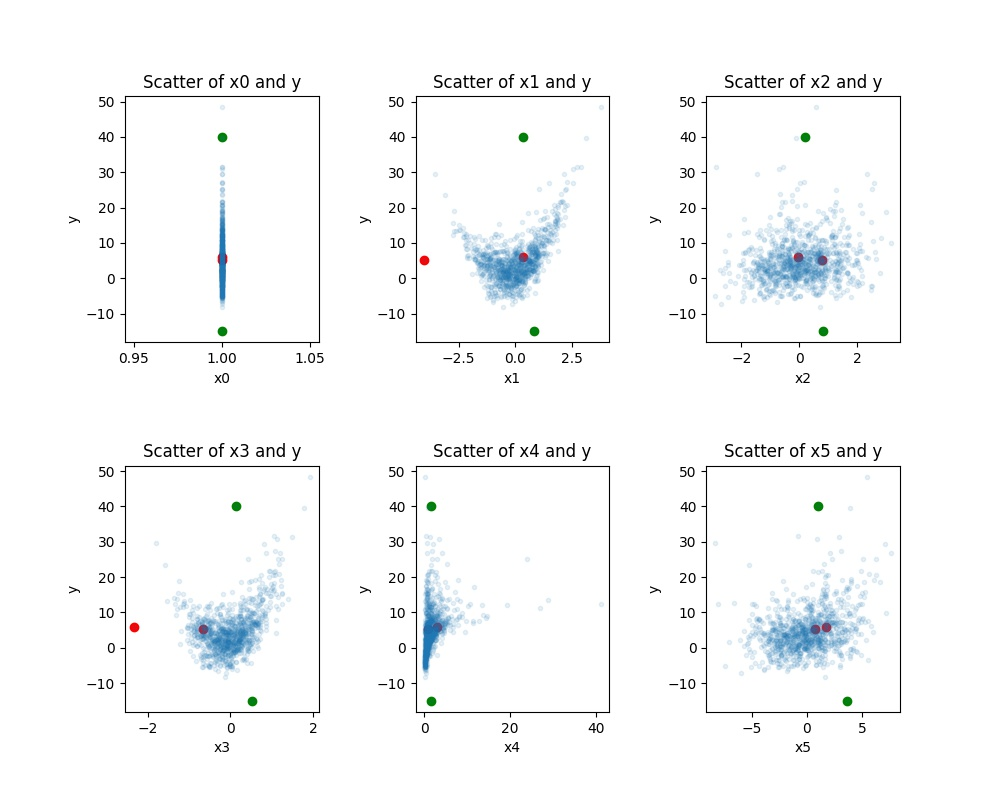
\includegraphics[width = 1\textwidth]{images/Scatter.jpg}
%\caption{fff}
%\end{figure}
\end{center}

Another problem we can observe is the nonlinearity between the response $y$ and the predictors $x_1$, $x_3$ and $x_4$. We will use nonlinear transformations to overcome this problem. Moreover, the pattern of the scatter plot of $x_1$ and $y$ is very similar to the patter of the scatter plot of $x_4$ and $y$, which indicates collinearity between $x_1$ and $x_4$. The collinearity can be detected by calculating the \textit{variance inflation factor} (VIF) and we will remove predictors of high VIF to remove collinearity. 

\subsection{Baseline model}
Before making any changes on the data set, we fit a multiple linear model with an unsurprisingly low $R^2$ score of $0.245$. Here is a summary of the results:\\
\begin{center}
$R^2 = 0.245$\\
 \begin{tabular}{lcccccc}
 \hline
           & \textbf{coef} & \textbf{std err} & \textbf{t} & \textbf{P$> |$t$|$} & \textbf{[0.025} & \textbf{0.975]}  \\
\midrule
\textbf{$x_0$} &       3.5888  &        0.202     &    17.758  &         0.000        &        3.192    &        3.985     \\
\textbf{$x_1$} &       1.3166  &        0.507     &     2.597  &         0.010        &        0.322    &        2.312     \\
\textbf{$x_2$} &       0.6121  &        0.577     &     1.060  &         0.289        &       -0.521    &        1.745     \\
\textbf{$x_3$} &       1.5163  &        0.812     &     1.868  &         0.062        &       -0.076    &        3.109     \\
\textbf{$x_4$} &       0.7321  &        0.064     &    11.495  &         0.000        &        0.607    &        0.857     \\
\textbf{$x_5$} &       0.1040  &        0.281     &     0.370  &         0.712        &       -0.448    &        0.656     \\
\bottomrule
\end{tabular}
\end{center}
We denote the estimated coefficients of $x_i$ as $\hat{\beta}_i$. The results show that the $p$ values of $\hat{\beta}_2$, $\hat{\beta}_3$ and $\hat{\beta}_5$ are large and their $95\%$ confidence intervals contains 0, which indicate these estimated coefficients are not statistically significant. This makes sense because $x_2$, $x_3$ and $x_5$ are linearly dependent. 

\subsection{Outliers}
Outliers are unusual response $y^i$ given the predictor $x^i$. To detect them, we compute the studentized residuals by dividing each residual by its standard error. Observations whose studentized residuals are greater than 3 in absolute value are likely to be outliers. This procedure was able to found $15$ outliers in our data set, including the two green outliers we added intentionally. We removed all the outliers, fitted the model again, and the resulting $R^2$ score was improved from the previous $0.245$ to $0.311$.
\begin{center}
$R^2 = 0.311$\\
\begin{tabular}{lcccccc}
\hline
           & \textbf{coef} & \textbf{std err} & \textbf{t} & \textbf{P$> |$t$|$} & \textbf{[0.025} & \textbf{0.975]}  \\
\midrule
\textbf{$x_0$} &       3.0225  &        0.174     &    17.369  &         0.000        &        2.681    &        3.364     \\
\textbf{$x_1$} &       0.7400  &        0.425     &     1.743  &         0.082        &       -0.093    &        1.573     \\
\textbf{$x_2$} &       0.4782  &        0.484     &     0.988  &         0.324        &       -0.472    &        1.428     \\
\textbf{$x_3$} &       1.8211  &        0.677     &     2.692  &         0.007        &        0.493    &        3.149     \\
\textbf{$x_4$} &       0.8932  &        0.060     &    14.959  &         0.000        &        0.776    &        1.010     \\
\textbf{$x_5$} &       0.2164  &        0.236     &     0.917  &         0.359        &       -0.246    &        0.679     \\
\bottomrule
\end{tabular}
\end{center}
Compared with the previous results, we found that after removing 15 outliers, the value of the estimated coefficients has been changed a lot and the standard errors were all reduced, which suggested the sensitivity of multiple linear regression models to outliers. Moreover, the $\hat{\beta}_3$ became statistically significant while $\hat{\beta}_1$ became statistically insignificant and $\hat{\beta}_2$ and $\hat{\beta}_4$ stay statistically insignificant. This is not a surprise as these four predictors are linearly dependent. 

\subsection{High-leverage points}

Observations with high-leverage have unusual value for predictor $x^i$. Leverage is a measure of how far away the values of predictors of an observation is from those of the other observations. It was computed as 
$$h_i = [H]_{ii}$$
with $$H = X(X^TX)^{-1}X^T$$
where $X$ is the design matrix.

If an observation has a leverage statistics greatly exceeds $n/m$, it is considered as a high-leverage point. We successfully spotted $16$ high-leverage points including the two red dots and removed all of them from our dataset. After fitting the model again, the $R^2$ statistics was improved from $0.311$ to $0.349$. 

\begin{center}
$R^2 = 0.349$\\
\begin{tabular}{lcccccc}
\hline
           & \textbf{coef} & \textbf{std err} & \textbf{t} & \textbf{P$> |$t$|$} & \textbf{[0.025} & \textbf{0.975]}  \\
\midrule
\textbf{$x_0$} &       2.1488  &        0.192     &    11.185  &         0.000        &        1.772    &        2.526     \\
\textbf{$x_1$} &       0.6565  &        0.442     &     1.484  &         0.138        &       -0.212    &        1.525     \\
\textbf{$x_2$} &       0.4168  &        0.483     &     0.863  &         0.388        &       -0.531    &        1.365     \\
\textbf{$x_3$} &       1.9357  &        0.724     &     2.673  &         0.008        &        0.515    &        3.357     \\
\textbf{$x_4$} &       1.5451  &        0.091     &    16.887  &         0.000        &        1.366    &        1.725     \\
\textbf{$x_5$} &       0.2368  &        0.236     &     1.004  &         0.316        &       -0.226    &        0.700     \\
\bottomrule
\end{tabular}
\end{center}
Again, the estimated coefficients have changed a lot after removing the high-leverage points and the statistical insignificancy of certain coefficients still exist. To further improve the model, we study the following scatter plots between each predictor and the residual, which clearly shows nonlinear relation between the residuals and $x_1$, $x_3$ and $x_4$.

\begin{center}
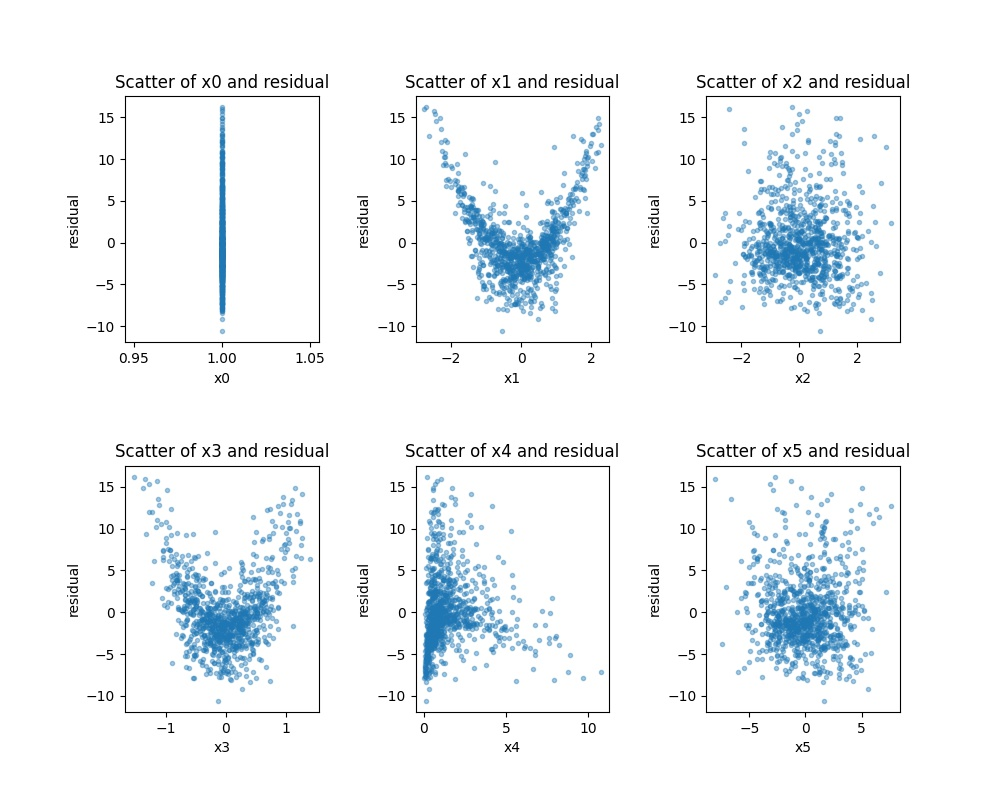
\includegraphics[width = 1\textwidth]{images/Scatter_cleaned.jpg}
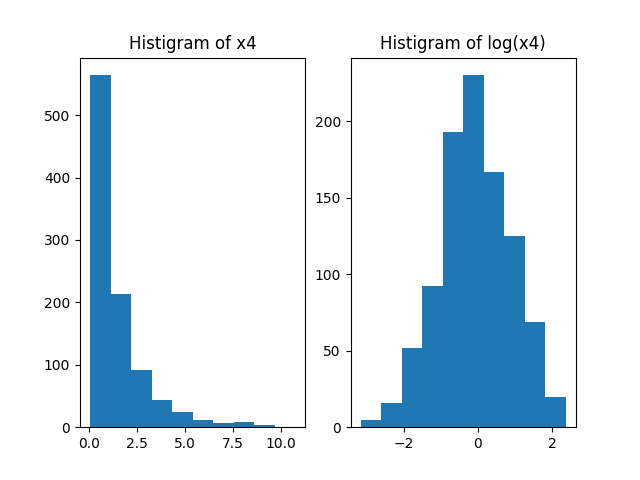
\includegraphics[width = .6\textwidth]{images/hist.png}
\end{center}
\subsection{Nonlinearity}
Firstly, since there are clear quadratic patterns in $x_1$ and $x_3$, we apply nonlinear transformations to them by adding two quadratic predictors $$x_6 = x_1^2 $$ and $$x_7 = x_3^2.$$ Secondly, the long tail in the histogram of $x_4$ suggests us to apply a logarithm transformation on it. The histogram plots above shows that applying a logarithm transformation turns a long tail distribution to a bell shaped distribution. So we add another predictor $$x_8 = \log x_4.$$ With these three nonlinear predictors added, we fit the model again and obtained a much higher $R^2$ score of $0.873$, which indicates that our model is able to explain $87.3\%$ of the variance in the response $y$. 
\begin{center}
$R^2 = 0.873$\\
\begin{tabular}{lcccccc}
\hline
           & \textbf{coef} & \textbf{std err} & \textbf{t} & \textbf{P$> |$t$|$} & \textbf{[0.025} & \textbf{0.975]}  \\
\midrule
\textbf{$x_0$} &       1.9303  &        0.145     &    13.357  &         0.000        &        1.647    &        2.214     \\
\textbf{$x_1$} &       1.8902  &        0.198     &     9.561  &         0.000        &        1.502    &        2.278     \\
\textbf{$x_2$} &       0.7209  &        0.214     &     3.368  &         0.001        &        0.301    &        1.141     \\
\textbf{$x_3$} &       0.8087  &        0.323     &     2.508  &         0.012        &        0.176    &        1.442     \\
\textbf{$x_4$} &       0.0257  &        0.077     &     0.334  &         0.739        &       -0.125    &        0.177     \\
\textbf{$x_5$} &       0.1355  &        0.105     &     1.297  &         0.195        &       -0.070    &        0.341     \\
\textbf{$x_6$} &       3.0566  &        0.099     &    31.023  &         0.000        &        2.863    &        3.250     \\
\textbf{$x_7$} &      -0.1853  &        0.336     &    -0.552  &         0.581        &       -0.844    &        0.473     \\
\textbf{$x_8$} &       2.9635  &        0.120     &    24.769  &         0.000        &        2.729    &        3.198     \\
\bottomrule
\end{tabular}
\end{center}

Now that the $R^2$ has been greatly improved to $0.873$, but the $p$-values of $\hat{\beta}_4$, $\hat{\beta}_5$ and $\hat{\beta}_7$ are still very high and they are statistically insignificant. A naive way will be simply removing those predictors or setting their coefficients to 0. To investigate it deeper, we study the VIF scores to see if there is any collinearity between the predictors. 


\begin{center}
\begin{table}
\hfill
\begin{tabular}{| c | c |}
\toprule
 feature &        VIF \\
\midrule
       $x_0$ &   5.578499 \\
       $x_1$ &   9.293768 \\
       $x_2$ &  12.733581 \\
       $x_3$ &   7.106871 \\
       $x_4$ &   3.627332 \\
       $x_5$ &  17.344735 \\
       $x_6$ &   3.578160 \\
       $x_7$ &   3.486127 \\
       $x_8$ &   3.621004 \\
\bottomrule
\end{tabular}
\hfill
\begin{tabular}{| c | c |}
\toprule
 feature &       VIF \\
\midrule
       $x_0$ &  5.578384 \\
       $x_1$ &  6.980102 \\
       $x_2$ &  1.004317 \\
       $x_3$ &  6.836414 \\
       $x_4$ &  3.623471 \\
       $x_6$ &  3.572963 \\
       $x_7$ &  3.476829 \\
       $x_8$ &  3.619983 \\
\bottomrule
\end{tabular}
\hfill
\begin{tabular}{| c | c |}
\toprule
 feature &       VIF \\
\midrule
       $x_0$ &  5.577329 \\
       $x_1$ &  1.041725 \\
       $x_2$ &  1.003236 \\
       $x_4$ &  3.623237 \\
       $x_6$ &  3.530439 \\
       $x_7$ &  3.453403 \\
       $x_8$ &  3.617884 \\
\bottomrule
\end{tabular}
\hfill
\begin{tabular}{|c|c|}
\toprule
 feature &       VIF \\
\midrule
       $x_0$ &  1.631185 \\
       $x_1$ &  1.041478 \\
       $x_2$ &  1.003019 \\
       $x_6$ &  3.518587 \\
       $x_7$ &  3.449602 \\
       $x_8$ &  1.001468 \\
\bottomrule
\end{tabular}
\hfill
\end{table}
\end{center}
\subsection{Collinearity}
After checking the VIF scores in the first table, we first removed the predictor $x_5$, which has the highest VIF score. This totally makes sense since by construction $x_5$ is a linear combination of $x_1$, $x_2$ and $x_3$. We then get the new VIF scores in the second table and found that $x_1$ and $x_3$ have similarly high VIF scores, which is reasonable because $x_3 =\frac 1 2 x_1 + \frac 1 5 \epsilon_1$ by construction. We choose to remove $x_3$ as it results to a higher $R^2$ score. After removing $x_3$ and $x_5$, we get the third table of VIF scores where the constant term $x_0$ has a relative high VIF score. But we are not going to remove it because we always need an intercept term in a linear regression model. We fit the model again and obtained a $R^2$ score of $0.872$, which is almost the same the previous $0.873$. This shows that removing $x_3$ and $x_5$ dose not cause any information lost. 

\begin{center}
$R^2 = 0.872$\\
\begin{tabular}{lcccccc}
\hline
           & \textbf{coef} & \textbf{std err} & \textbf{t} & \textbf{P$> |$t$|$} & \textbf{[0.025} & \textbf{0.975]}  \\
\midrule
\textbf{$x_0$} &       1.9255  &        0.145     &    13.273  &         0.000        &        1.641    &        2.210     \\
\textbf{$x_1$} &       2.4629  &        0.066     &    37.063  &         0.000        &        2.332    &        2.593     \\
\textbf{$x_2$} &       0.9817  &        0.060     &    16.274  &         0.000        &        0.863    &        1.100     \\
\textbf{$x_4$} &       0.0242  &        0.077     &     0.313  &         0.754        &       -0.127    &        0.176     \\
\textbf{$x_6$} &       3.0820  &        0.098     &    31.367  &         0.000        &        2.889    &        3.275     \\
\textbf{$x_7$} &      -0.2402  &        0.335     &    -0.716  &         0.474        &       -0.898    &        0.418     \\
\textbf{$x_8$} &       2.9580  &        0.120     &    24.637  &         0.000        &        2.722    &        3.194     \\
\bottomrule
\end{tabular}
\end{center}

The table above shows high $p$ values of $\hat{\beta}_4$ and $\hat{\beta}_7$. We remove $x_4$ first as it has a higher $p$ value and see the resulting $\hat{\beta}_7$ is still statistically insignificant. So we also remove $x_7$ and obtained a model still with $R^2 = 0.872$. This makes sense because we know the response $y$ dose not depend on $x_4$ linearly and $x_7 = x_3^2 \approx \frac 1 4 x_1^2 = \frac 1 4 x_6.$ Also, the last VIF table above shows a comparable large VIF scores between $x_6$ and $x_7$, indicating linearity between them. 
\begin{center}
$R^2 = 0.872$\\
\begin{tabular}{lcccccc}
\hline
                  & \textbf{coef} & \textbf{std err} & \textbf{t} & \textbf{P$> |$t$|$} & \textbf{[0.025} & \textbf{0.975]}  \\
\midrule
\textbf{$x_0$} &       1.9547  &        0.077     &    25.266  &         0.000        &        1.803    &        2.107     \\
\textbf{$x_1$} &       2.4569  &        0.066     &    37.275  &         0.000        &        2.328    &        2.586     \\
\textbf{$x_2$} &       0.9824  &        0.060     &    16.301  &         0.000        &        0.864    &        1.101     \\
\textbf{$x_6$} &       3.0219  &        0.053     &    57.116  &         0.000        &        2.918    &        3.126     \\
\textbf{$x_8$} &       2.9898  &        0.063     &    47.365  &         0.000        &        2.866    &        3.114     \\
\bottomrule
\end{tabular}
\end{center}
After removing $x_4$ and $x_7$, all the estimated coefficients are statistically significant and $R^2 = 0.872$ is also pretty acceptable. Recall that our under truth model is 
\begin{align*}\label{eq2}
y &= 2 x_0 + \frac 5 2 x_1 + 3 x_1^2 + x_2 + 3\log{x_4} + 3 x_2 \epsilon +  2 \epsilon + \frac 1 5 \epsilon_1 \\
&= 2 x_0 + \frac 5 2 x_1+ x_2 + 3 x_6  + 3 x_8+ 3 x_2 \epsilon +  2 \epsilon + \frac 1 5 \epsilon_1.
\end{align*}
The estimated coefficients are really close to the true coefficients. We know this is a perfect estimation already. But in reality, one may not be satisfied with $R^2 = 0.872$ and try to explore the residuals further.

\begin{center}
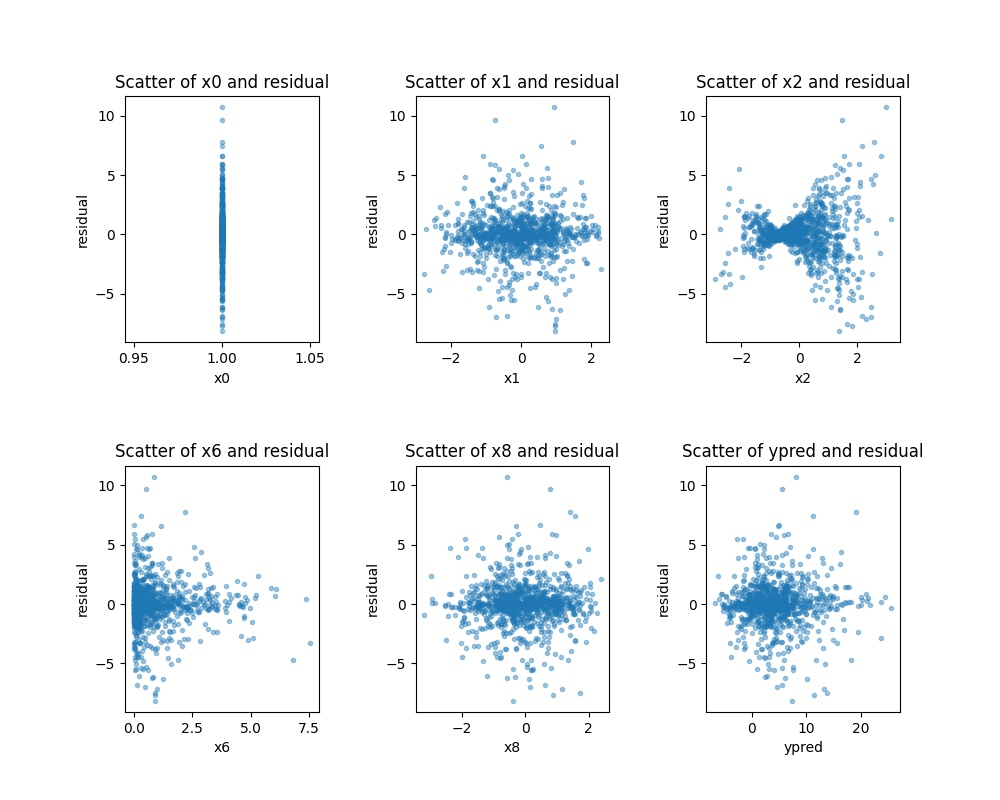
\includegraphics[width = 1\textwidth]{images/Scatter_res.jpg}
\end{center}
\subsection{Heteroscedasticity}
The scatter plots indicates that the variance of our residual depends on $x_2$ and $x_6$ instead of staying constant. This phenomena is called heteroscedasticity. We applied weighted least square regression where weights are calculated as the squared reciprocal of the residuals of a regression of the residual from the previous model and $x_2$ and $x_6$. In this way, observations with a high residual will have a low weight while those with a low residual will have a high weight. The weighted model is trying to fit the observations with high weights better and put less efforts on fitting those points with low weights. The results show a high $R^2 = 0.943$, which seems to be very exciting. However, the estimated parameters are far away from the true parameters and the standard errors are also high compared with the results in the previous section. We first thought this is because the weighted model is able to explain the error terms better. However, after digging deep we found the reason is that most of observations have a very low weight while a few have an extremely high weight ($\approx 6 \times 10^4$) and the $R^2$ score is calculated with weights, making the weighted Total Sum of Squares extremely large and leading to a high $R^2$ score. (The formulas of the weighted $R^2$ is provided in \nameref{marker}.) Therefore, we should not use $R^2$ score as the unique measure of the goodness of a model. 
\begin{center}
$R^2 = 0.943$\\
\begin{tabular}{lcccccc}
\hline
           & \textbf{coef} & \textbf{std err} & \textbf{t} & \textbf{P$> |$t$|$} & \textbf{[0.025} & \textbf{0.975]}  \\
\midrule
\textbf{$x_0$} &       2.5157  &        0.228     &    11.026  &         0.000        &        2.068    &        2.963     \\
\textbf{$x_1$} &       3.1952  &        0.049     &    65.102  &         0.000        &        3.099    &        3.292     \\
\textbf{$x_2$} &       0.4977  &        0.125     &     3.980  &         0.000        &        0.252    &        0.743     \\
\textbf{$x_6$} &       2.5049  &        0.036     &    69.089  &         0.000        &        2.434    &        2.576     \\
\textbf{$x_8$} &       3.0130  &        0.041     &    73.445  &         0.000        &        2.932    &        3.093     \\
\bottomrule
\end{tabular}
\end{center}
Even though the model fitted by Weighted Least Square is not very accurate, the following residual scatter plots show that the variance of the residual is a little bit more steady with respect to $x_2$. 

\begin{center}
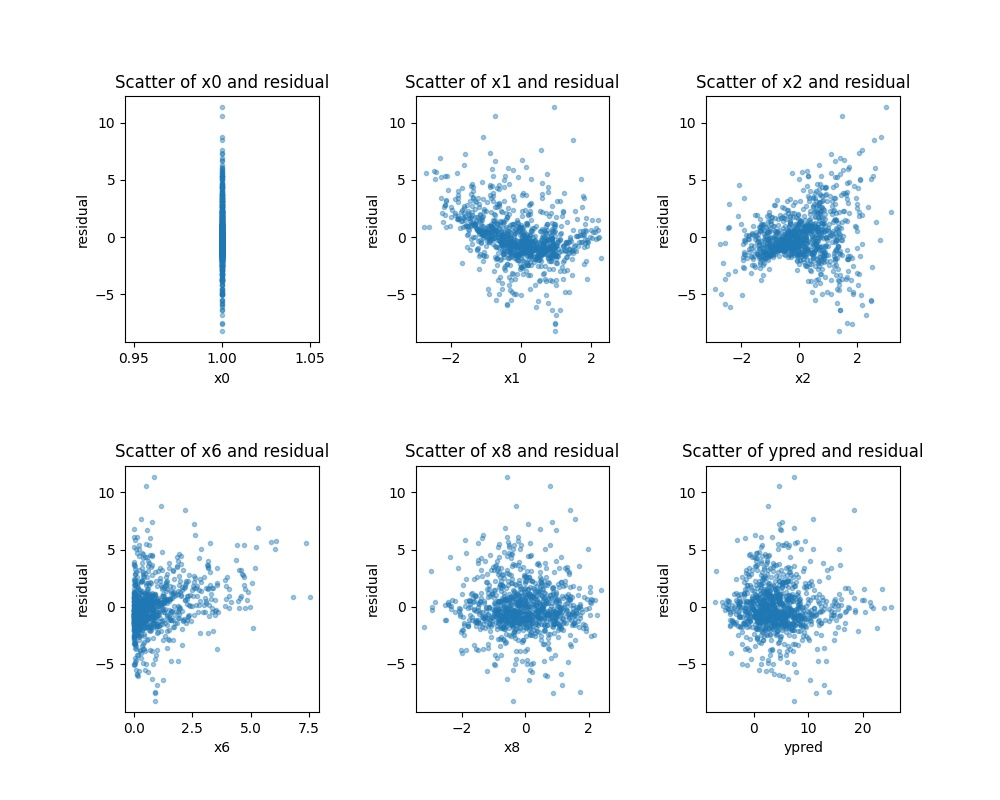
\includegraphics[width = 1\textwidth]{images/Scatter_res1.jpg}
\end{center}

%\begin{enumerate}
%\item Nonlinearity of the response-predictor relationships. 
%
%We will fit our model and make a plot of fitted values VS residuals to see if there is a clear nonlinear pattern in residuals. If so, we should consider creating nonlinear transformation of predictors, such as $\log x_i$, $x_ix_j$ and $x_i^2$ for our model. 
%
%\item Non-constant variance of error terms.
%
%Again, we will fit our model and make a plot of fitted values VS residuals to check if the variance of the residuals changes. If so, we can consider either make a nonlinear transformation of the response $Y$ or fit our model by weighted least squares, with weights proportional to inverse variance. 
%
%\item Outliers.
%
%\item Collinearity.
%
%We will compute the Variance Inflation Factor (VIF) of each predictor to check collinearity. A VIF value that is greater than 5 or 10 indicates a problematic amount of collinearity. We can either remove the problematic predictor or take an average of standardized versions of the collinear predictors in order to create a new variable. 
%
%\item Correlation of the error terms. 
%
%If two errors are correlated, then knowing one error will help us to guess the other error.  We can analyze the plot of the residuals and check if there is tracking to see if there is correlation between the residuals. We won't go deep to seek for solutions to solve this problem. In practice, the experiments should be carefully designed to ensure uncorrelated errors. 
%
%%\item Dependence of the predictors and error terms.
%%\item Nonzero error means.
%\end{enumerate}
\newpage
\section{Evaluation and Final Results}
\label{marker}
Our methods and results can be summarized in the following figure:
\begin{center}
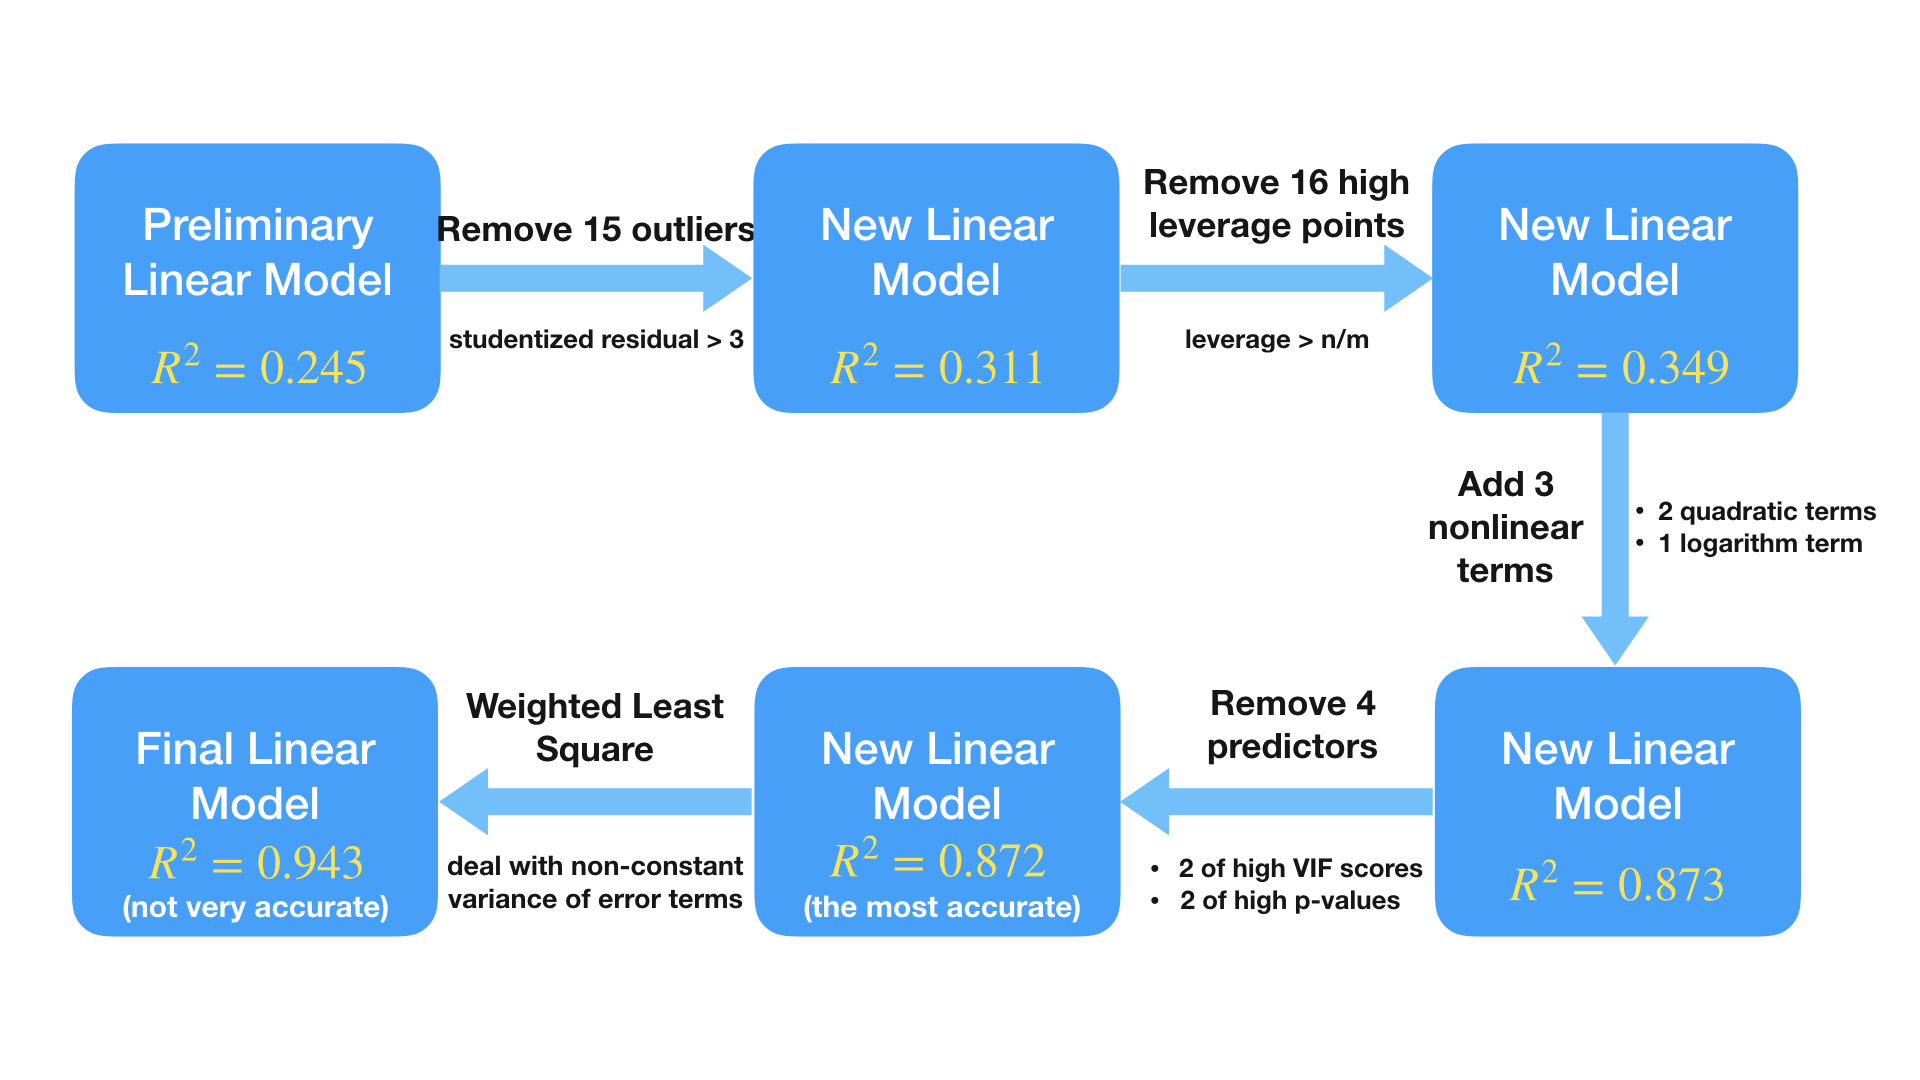
\includegraphics[width = .89\textwidth]{images/work_flow.png}
\end{center}
We evaluated our linear regression models using $R^2$ statistics given in the following formulas:
\begin{itemize}
\item Residual Sum of Squares: $$RSS = \sum_{i=1}^n (y_i - \hat{y_i})^2$$
%\item Residual Standard Error: $RSE = \sqrt{\frac{RSS}{n-p-1}}$ where $n-p-1$ is the degree of freedom since we have $n$ data points and $p+1$ parameters. $RSE$ measures the lack of fit of the models to the data. It is an absolute measure, which means it depends on the scale of $y_i$. We can use it together with the $R^2$ statistic. 
\item Total Sum of Squares: $$TSS = \sum_{i=1}^n (y_i - \bar{y})^2$$
\item $R^2$ statistics: $$R^2 = \frac{TSS - RSS}{TSS} = 1 - \frac{RSS}{TSS}$$ 
The $R^2$ statistics measures the proportion of variance explained by the fitted model when we apply ordinary least square to fit a linear regression model. For model fitted by weighted least square, the $R^2$ statistics is calculated using a weight vector $w$ in the following way:

\item The weighted Residual Sum of Squares: $$RSS_w = \sum_{i=1}^n w_i (y_i - \hat{y_i})^2$$
%\item Residual Standard Error: $RSE = \sqrt{\frac{RSS}{n-p-1}}$ where $n-p-1$ is the degree of freedom since we have $n$ data points and $p+1$ parameters. $RSE$ measures the lack of fit of the models to the data. It is an absolute measure, which means it depends on the scale of $y_i$. We can use it together with the $R^2$ statistic. 
\item The weighted Total Sum of Squares: $$TSS_w = \sum_{i=1}^n w_i (y_i - \bar{y}_w)^2$$
with $$\bar{y}_w = \frac{\sum_{i=1}^n w_i y_i} {\sum_{i=1}^n w_i} .$$
\item The weighted $R^2$ statistics: $$R^2_w = \frac{TSS_w - RSS_w}{TSS_w} = 1 - \frac{RSS_w}{TSS_w}$$ 
As we mentioned before, the weighted $R^2$ might be very close to 1 when $w$ has large entries which makes the $TSS_w$ very large. So we should not use it as the unique measure of the goodness of a fitted model. Instead, we can also check the standard errors and $p$-values of the estimated coefficients. 
\end{itemize} 


\begin{thebibliography}{100}
 
 \bibitem{rmat1}  Gareth James, Daniela Witten, Trevor Hastie, Robert Tibshirani. An Introduction to Statistical Learning : with Applications in R. In \emph{New York :Springer}, 2013.
 
 \bibitem{rmat2}  Seabold, Skipper, and Josef Perktold. statsmodels: Econometric and statistical modeling with python. \emph{Proceedings of the 9th Python in Science Conference}. 2010.

 \bibitem{rmat3} \href{https://online.stat.psu.edu/stat501/lesson/13}{STAT 501 online course materials website, PennState}


\end{thebibliography}
\end{document}

